%
%  Vincent Yannello
%
\documentclass[12pt,fullpage]{article}
\usepackage{fullpage}
\usepackage{psfrag}                                          % LaTeX graphics tool
\usepackage{pslatex}                                         % avoids the default cmr font
\usepackage{graphicx}                                        % graphics package 
\usepackage{epsfig}                                          % figures
\usepackage{hyperref}
\usepackage{color}

\begin{document}

\noindent
{\bf Pareto distribution} (from \color{blue}\url{http://www.math.wm.edu/~leemis/chart/UDR/UDR.html}\color{black})

\noindent
The shorthand $X \sim {\rm Pareto}(\lambda, \kappa)$ is used to indicate that the
random variable $X$ has the Pareto distribution with parameters $\lambda$ and $\kappa$.
A Pareto random variable $X$ with positive parameters $\lambda$ and~$\kappa$ has probability density function 
$$
f(x) = {\frac {\kappa\,{\lambda}^{\kappa}}{{x}^{\kappa+1}}} \qquad \qquad x > \lambda.
$$
The Pareto distribution has traditionally been used to model the distribution of income,
where $\lambda$ is a minimum wage and $\kappa$ models the distribution of the income.
The Pareto distribution can also be used to model the lifetime of an object with a warranty
period $\lambda$ or the duration of a strike with minimum duration $\lambda$.
The probability density function with $\lambda = 1$ and two different values of $\kappa$ is illustrated below.
{\begin{figure}[h!]
\begin{center}
\psfrag{lab1}{$\kappa = 1$}
\psfrag{lab2}{$\kappa = 4$}
\psfrag{labx}{$x$}
\psfrag{labf}{$f(x)$}
\includegraphics[width=3.2in]{ParetoPlot.ps}
\end{center}
\end{figure}}\\
The cumulative distribution function on
the support of $X$ is
$$
F(x) = P(X \le x) = 1 - \left(\frac{\lambda}{x}\right)^{\kappa}  \qquad \qquad x > \lambda.
$$
The survivor function on the support of $X$ is
$$
S(x) = P(X \ge x) = \left(\frac{\lambda}{x}\right)^{\kappa}  \qquad \qquad x > \lambda.
$$
The hazard function on the support of $X$ is
$$
h(x) = \frac{f(x)}{S(x)} = \frac{\kappa}{x} \qquad \qquad x > \lambda.
$$
The cumulative hazard function on the support of $X$ is
$$
H(x) = - \ln S(x) = -\kappa (\ln \lambda - \ln x) \qquad \qquad x > \lambda.
$$
The inverse distribution function of $X$ is
$$
F ^ {-1}(u) = \lambda(1 - u)^{-1/\kappa} \qquad \qquad 0 < u < 1.
$$
The median of $X$ is
$$
\lambda 2^{1/\kappa}.
$$
The moment generating function of $X$ is
$$
M(t) = E\left[ e ^ {tX} \right] = \kappa (-\lambda t)^{\kappa}\Gamma(-\kappa, -\lambda t) \qquad \qquad -\infty < t < \infty.
$$
The characteristic function of $X$ is
$$
\phi(t) = E\left[ e ^ {itX} \right] =  \kappa (-\lambda it)^{\kappa}\Gamma(-\kappa, -\lambda it) \qquad \qquad -\infty < t < \infty.
$$
The population mean, variance, skewness, and kurtosis of $X$ are
$$
\qquad E[X] = \frac{\kappa \, \lambda} {\kappa - 1}\ \  {\rm for}\ \kappa > 1 \qquad \qquad \qquad \qquad
V[X] = \frac{\kappa \, \lambda ^ 2}{(\kappa - 1) ^ 2(\kappa - 2)}\ \ {\rm for}\ \kappa >2 \qquad \qquad
$$
$$
E\left[ \left( \frac{X - \mu}{\sigma} \right) ^ {\kern -0.08 em 3} \right] = 2 \, \frac{\kappa+1}{\kappa - 3} \sqrt{\frac{\kappa - 2}{\kappa}}\, {\rm for}\ \kappa >3 \qquad \qquad 
E\left[ \left( \frac{X - \mu}{\sigma} \right) ^ {\kern -0.08 em 4} \right] =  \frac{3(\kappa - 2)(3\kappa^3 + \kappa + 2)}{\kappa(\kappa-3)(\kappa-4)}\ \ {\rm for}\ \kappa>4.
$$

\vspace{0.1in}

\noindent
{\bf APPL verification:}
The APPL statements
\begin{verbatim}
X := ParetoRV(lambda, kappa);
CDF(X);
SF(X);
HF(X);
CHF(X):
IDF(X);
assume(kappa > 1);
Mean(X);
assume(kappa > 2);
Variance(X);
assume(kappa > 3);
Skewness(X);
assume(kappa > 4);
Kurtosis(X);
MGF(X);
\end{verbatim}
verify the cumulative distribution function, survivor function, hazard function, cumulative hazard function, and inverse distribution function.
Some of the population moments are expressed as limits. 
\end{document}
